This section presents the simulation of the \textit{Poiseuille} flow 
in half of the domain. Thus, the free-slip condition is required on 
the axis of symmetry. The \ref{half poiseuille} presents schematically 
this flow with the specified axis of symmetry and the expected velocity 
field.

\begin{figure}[H]
\begin{center}
\begin{tikzpicture}[scale=1.2]
 \draw [pattern=north east lines] (0,1) -- (0,1.1) -- (5,1.1) -- (5,1) -- cycle;
 \draw [dashed] (-0.3,0.0) to (5.3,0.0);

 \draw [->,thick] (-2,-0.1)--(-2,1.5) node[left] {$y$};
 \draw [->,thick] (-2.1,0)--(-0.5,0) node[below] {$x$};

 \draw [->,thick] (5.4,0.0)--(6.1,0.0);
 \node [draw=none] at (7.1,0.0) {$symmetry$};
 
 \draw [dotted] (2.5,0.0) to (2.5,1.0);
 \draw  (2.8,0.0) to [bend right=20] (2.5,1.0);
 
 \draw [->,thick] (2.5,0.0) to (2.8,0.0);
 \draw [->,thick] (2.5,0.3) to (2.78,0.3);
 \draw [->,thick] (2.5,0.6) to (2.71,0.6);
 \draw [->,thick] (2.5,0.85) to (2.6,0.85);
\end{tikzpicture}
\end{center}
\caption{Half Poiseuille flow}
\label{half poiseuille}
\end{figure}

\noindent
The velocity profile equation is shown below:

\begin{equation}
 u = u_{max} \big[ 1 - \frac{y^{2}}{L^{2}} \big]
\end{equation}


\medskip
where $u_{max}$ is maximum velocity and its value is 
$u_{max} = 1.5$, $L$ is non-dimensional length 
between the plates and its value is 
$L = 1$
and $y$ is the vertical coordinates and it varies 
between $y = \big[ 0,1 \big]$.
The domain was discretized using a linear triangular mesh
with 3835 nodes and 7299 elements.


\medskip
The \ref{velocidade half poiseuille} shows the unsteady velocity profile
when $Re=100$, in addition to the comparison between the 
numerical and analytical solutions in the steady state of
proposed problem. It is possible to observe that the numerical
solution converges to the analytical solution when the flow
becomes steady state.



\begin{figure}[H]
     \centering
     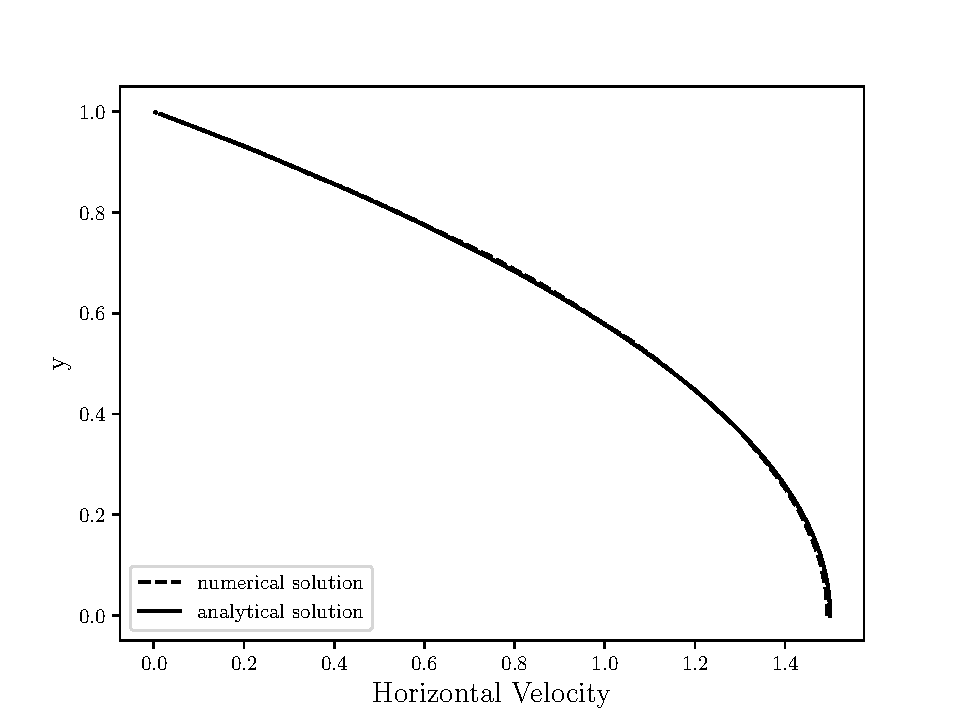
\includegraphics[scale=1]{./02_chaps/cap_validation/figure/half_poiseuille_velocity.pdf}\\
     \medskip
     \caption{
Unsteady velocity profile when $Re=100$ and the comparison between
the numerical and analytical solution for Half Poiseuille flow.} 
     \label{velocidade half poiseuille}
\end{figure}

